\documentclass[journal]{vgtc}                % final (journal style)
%\documentclass[review,journal]{vgtc}         % review (journal style)
%\documentclass[widereview]{vgtc}             % wide-spaced review
%\documentclass[preprint,journal]{vgtc}       % preprint (journal style)
%\documentclass[electronic,journal]{vgtc}     % electronic version, journal

%% Uncomment one of the lines above depending on where your paper is
%% in the conference process. ``review'' and ``widereview'' are for review
%% submission, ``preprint'' is for pre-publication, and the final version
%% doesn't use a specific qualifier. Further, ``electronic'' includes
%% hyperreferences for more convenient online viewing.

%% Please use one of the ``review'' options in combination with the
%% assigned online id (see below) ONLY if your paper uses a double blind
%% review process. Some conferences, like IEEE Vis and InfoVis, have NOT
%% in the past.

%% Please note that the use of figures other than the optional teaser is not permitted on the first page
%% of the journal version.  Figures should begin on the second page and be
%% in CMYK or Grey scale format, otherwise, colour shifting may occur
%% during the printing process.  Papers submitted with figures other than the optional teaser on the
%% first page will be refused.

%% These three lines bring in essential packages: ``mathptmx'' for Type 1
%% typefaces, ``graphicx'' for inclusion of EPS figures. and ``times''
%% for proper handling of the times font family.

\usepackage{mathptmx}
\usepackage{graphicx}
\usepackage{times}
\usepackage{float}
\usepackage{bbold}



%% We encourage the use of mathptmx for consistent usage of times font
%% throughout the proceedings. However, if you encounter conflicts
%% with other math-related packages, you may want to disable it.

%% This turns references into clickable hyperlinks.
\usepackage[bookmarks,backref=true,linkcolor=black]{hyperref} %,colorlinks
\hypersetup{
  pdfauthor = {},
  pdftitle = {},
  pdfsubject = {},
  pdfkeywords = {},
  colorlinks=true,
  linkcolor= black,
  citecolor= black,
  pageanchor=true,
  urlcolor = black,
  plainpages = false,
  linktocpage
}
\usepackage[hyphenbreaks]{breakurl}

%% If you are submitting a paper to a conference for review with a double
%% blind reviewing process, please replace the value ``0'' below with your
%% OnlineID. Otherwise, you may safely leave it at ``0''.
\onlineid{0}

%% declare the category of your paper, only shown in review mode


%% allow for this line if you want the electronic option to work properly


%% In preprint mode you may define your own headline.
%\preprinttext{To appear in an IEEE VGTC sponsored conference.}

%% Paper title.

\title{DEEP COMPRESSION: COMPRESSING DEEP NEURAL NETWORKS WITH PRUNING AND QUANTIZATION}
%\subtitle{Neural Network project, A.Y. 2018/2019}

%% This is how authors are specified in the journal style

%% indicate IEEE Member or Student Member in form indicated below
\author{Angelo Catalani 1582230}
\abstract{
Neural Network are both computationally intensive and memory intensive, making them difficult to deploy on embedded systems with limited hardware resources.\\Compressing a neural network with pruning and quantization with low loss of accuracy is the aim of this project }
%%%%%%%%%%%%%%%%%%%%%%%%%%%%%%%%%%%%%%%%%%%%%%%%%%%%%%%%%%%%%%%%
%%%%%%%%%%%%%%%%%%%%%% START OF THE PAPER %%%%%%%%%%%%%%%%%%%%%%
%%%%%%%%%%%%%%%%%%%%%%%%%%%%%%%%%%%%%%%%%%%%%%%%%%%%%%%%%%%%%%%%%
%  \teaser{
% \centering
% \includegraphics[width=16cm]{}
%  \caption{The whole project in a picture}
%  }
\begin{document}

%% The ``\maketitle'' command must be the first command after the
%% ``\begin{document}'' command. It prepares and prints the title block.

%% the only exception to this rule is the \firstsection command
\maketitle
\section{Introduction}
I have taken into consideration the following papers:
\begin{enumerate}
\item \cite{p1} : deals with specific pruning issues: regularization terms, threshold choice, and  parameter co-adaption
\item \cite{p2} : is the sequel of the previous paper : pruning and quantization
\end{enumerate}
\section{Pruning}
The pruning technique I have implemented as described in the papers consists of three steps :
\begin{enumerate}
\item train connectivity : the neural network is trained for a given number of epochs
\item prune connection : remove all the weights below a threshold
\item train the weights : re-train the reduced neural network to learn the final weights and repeat from step 2
\end{enumerate}
\begin{figure}[H]
	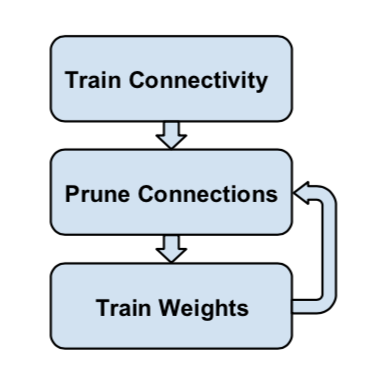
\includegraphics[width=30mm,scale=0.5]{prune-view}
	\caption{Pruning process}
\end{figure}
It is significant to note that:
\begin{enumerate}
\item the first step is conceptually different from the way a neural network is normally trained because in this step we are interested in finding the important connection rather than the final weights
\item retraining the pruned neural network is necessary for the accuracy since after the remotion of some connection (step 2),in general the accuracy will drop
\item pruning works under the hypothesis that the network is over-parametrized so that it solves not only memory/complexity issues but also can reduce the risk of overfitting
\end{enumerate}
The regularization terms used in the loss function, tends to lower the magnitude of the weight matrices, so that more weights will be close to zero and good candidates for being pruned.\\In particular, I have chosen L2 regularization because gives better results than L1(\cite{p1}).\\Deep neural network can be affected by the vanishing gradient problem.Even if \cite{p1} does not deals directly with that problem it notes that when a neural network struggles to update its weights consistently, it will not be able to recover from pruning of some neurons during the iterative pruning train. \\To deals with this issue, as written in  \cite{p1} I have pruned the convolutional layers and the dense layers on different iterations, so that the error caused by the pruning at each iteration is attenuated.\\In \cite{p1}, the threshold value is obtained as a quality parameter multiplied by the standard deviation of a layer's weights.\\This choice is justified by the fact that as it is the case of my experiments, the weights of a dense/convolutional layers are distributed as a gaussian of zero mean so that the weights in the range of the positive and negative standard deviation are 68\% of the total.
\begin{figure}[H]
	\hspace*{-1cm}
	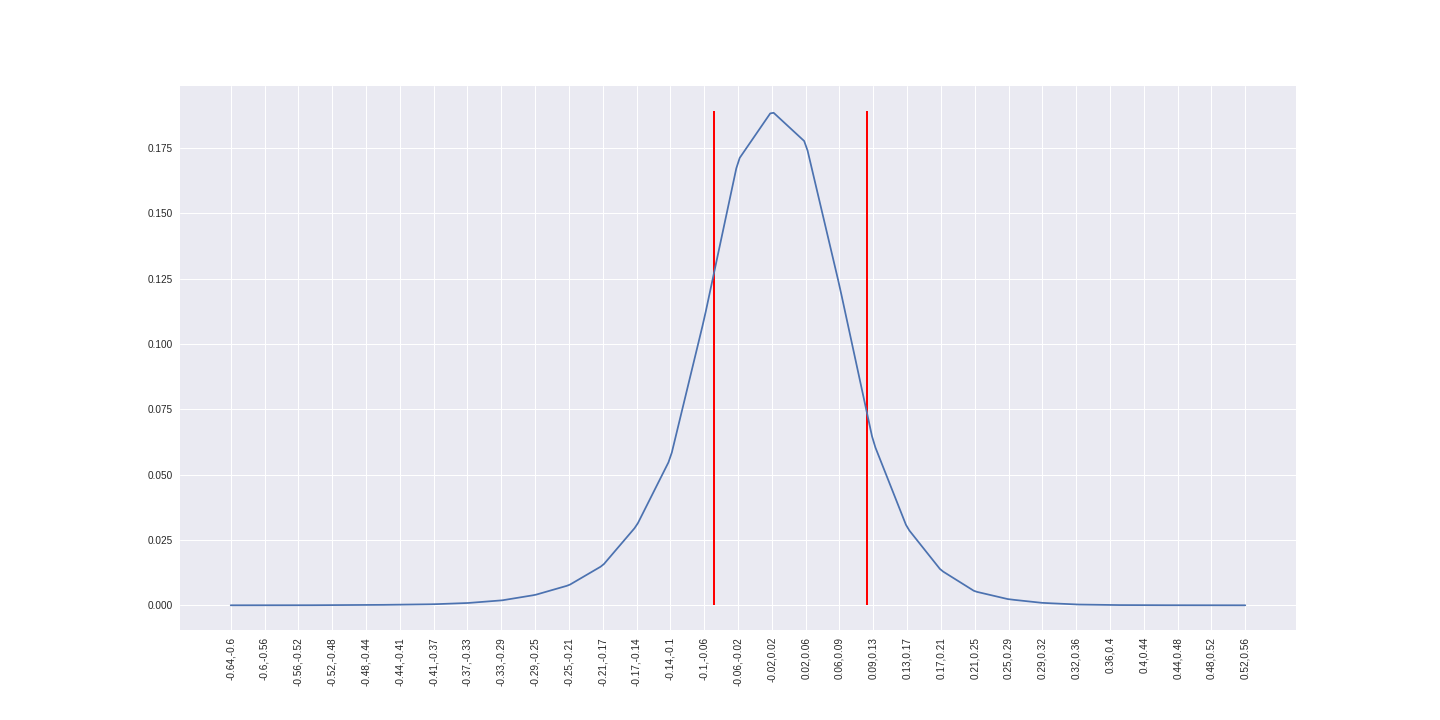
\includegraphics[width=90mm,scale=0.7]{weigth-dis}
	\caption{Weight distribution  (with +/- std in red) before pruning for a dense layer of Lenet300-100 }
\end{figure}
\section{Quantization And Weight Sharing}
This section is described in \cite{p2}.\\After the network has been pruned, the network is further compressed by reducing the number of bits to represent the single weights.\\In particular I have applied k-means (with 1 dimensional data) to the weights of each layer so that the new weights of the layer are the centroids to which the original weights belong to.\\Crucial to this step is the choice of k and the centroid initialization.\\The choice of k is a consequence of the number of bits used in this step : if we want to compress the layers weights to n bits, we can use up to $2^{n}$ centroids.\\The tradeoff between accuracy-compression is due to the number of bits used : the more the bits, the more the accuracy, the more the space required.\\The paper describes 3 different technique regarding the centroid initialization:
\begin{enumerate}
\item forgy : random choice among the weights 
\item density-based : consider the cumulative distribution of weights (cdf) and takes the x-values at different fixed y-values (cdf)
\item linear : consider equal sized intervals as centroids between the minimum and maximum weight
\end{enumerate}
In order to fully differentiate the initialization methods, it is important to note  the weights of a single layer are distributed as a bimodal distribution after the pruning : this means that :
\begin{enumerate}
\item forgy and density-based will place the weights around the two peaks because it is where weights are concentrated and the cdf varies the most. The drawback is that very few centroids will have large absolute value which results in poor representation of the few large weights.
\item linear equally space the range of weights, so it does not suffer from the previous problem
\end{enumerate}
\begin{figure}[H]
	\hspace*{-1cm}
	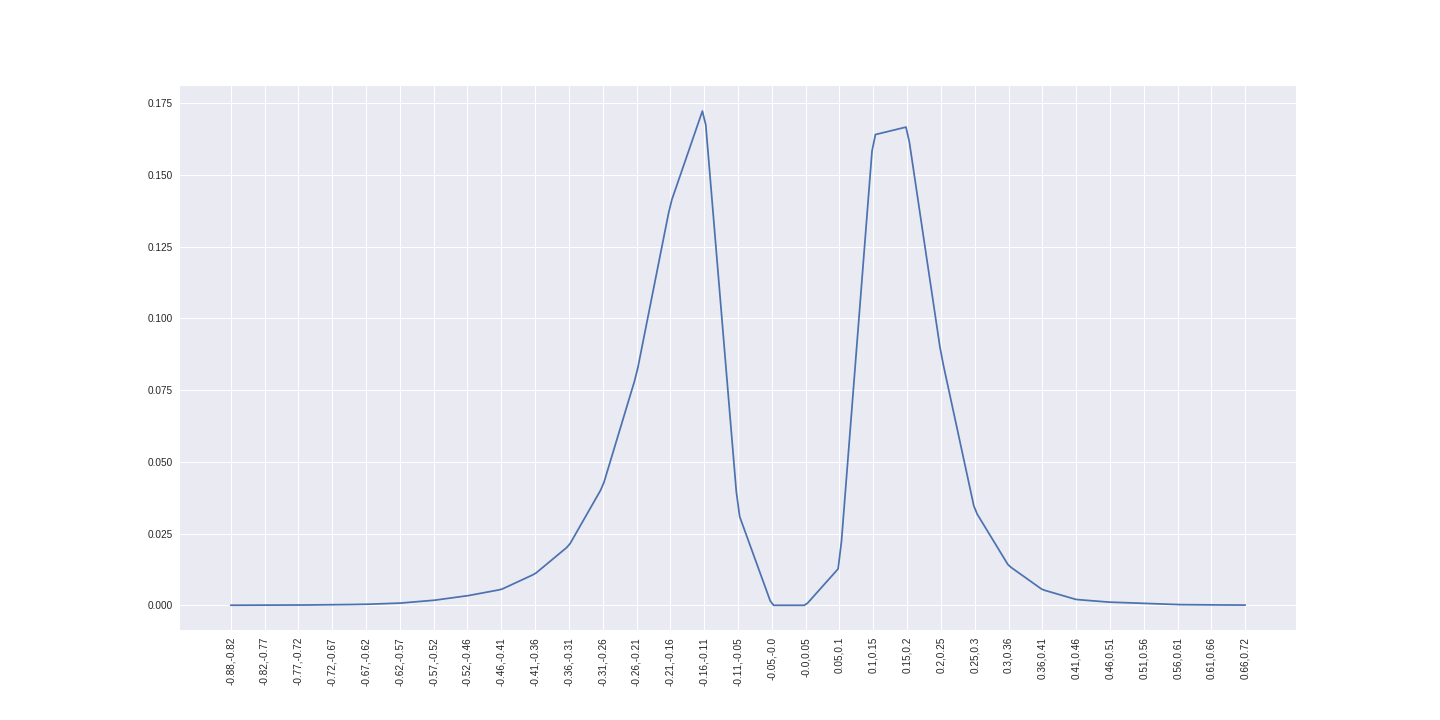
\includegraphics[width=90mm,scale=0.7]{weights-after-pruning}
	\caption{Weight distribution  after pruning for a dense layer of Lenet300-100 }
\end{figure}
\begin{figure}[H]
	\hspace*{-1cm}
	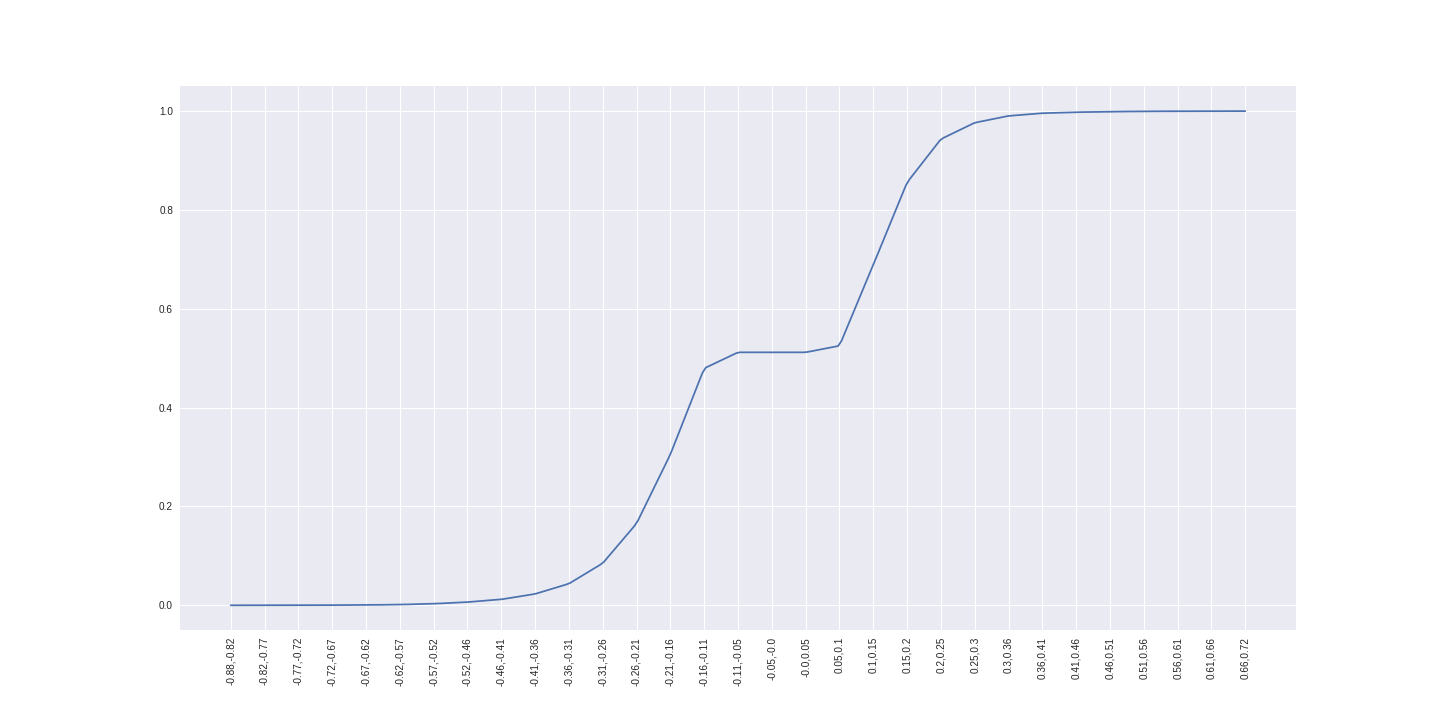
\includegraphics[width=90mm,scale=0.7]{cdf}
	\caption{Cumulative distribution for a dense layer of Lenet300-100 }
\end{figure}

At the end of this process, each layer will have at most $2^{n}$ different values.\\In addition to this, the paper perform the fine tuning of the centroids $C_k$ in the following way :
\begin{enumerate}
\item compute normally the gradient of the loss with respect to the weights : $\frac{\partial L}{\partial W_{ij}}$
\item sum the gradients whose weights belongs to a given centroid : $\frac{\partial L}{\partial C_{k}}=\sum\limits_{i,j}\frac{\partial L }{\partial W_{ij}}\cdot \mathbb{1}(I_{ij}=k) ]$
\end{enumerate}
I have not implemented the fine tuning of the centroids because:
\begin{enumerate}
\item the loss of accuracy after quantization is almost inexistent with respect to the pruned model
\item the latency is eccessive : for each single batch in every epoch, I should have scanned all the gradients
\end{enumerate}

\section{Experiment}
I have run my experiment on the MNIST classification problem using the Colaboratory , with the neural networks named : LeNet300-100 and LeNet5.\\Each element in the dataset is an image of size : 28 x 28 and the output class is a vector of 10 values obtained using the one hot encoding.\\LeNet300-100 has in total:
\begin{enumerate}
\item  a fully connected layer of size 300 : $28\cdot 28 \cdot 300 = 235200$ weights plus $300$ bias weights
\item  a fully connected layer of size 100 : $300\cdot 100 = 30000$ weights plus $100$ bias weights
\item  a fully connected layer of size 10 : $10\cdot 100 = 1000$ weights plus $4$ bias weights
\end{enumerate}
The second one :
\begin{enumerate}
\item  a convolutional layer with 20 filters of shape 5 by 5 : $20\cdot 5 \cdot 5 \cdot 1= 500$ weights plus $20$ bias weights
\item  a convolutional layer with 50 filters of shape 5 by 5 : $50\cdot 5 \cdot 5 \cdot 20= 25000$ weights plus $50$ bias weights
\item  a fully connected layer of size 256 : $256\cdot 2450 = 627200$ weights plus $256$ bias weights (2450 is the flattened output of the previous layer)
\item a fully connected layer of size 10 : $10\cdot256=2560$ weights plus $10$ bias weights
\end{enumerate}
The loss function is the categorical cross entropy with L2 regularization and the optimizer algorithm is Adam with $0.001$ as learning rate.
\subsection{Test 1}
It is executed with LeNet300-100 with 200 epochs for normal training and 30 epochs for pruning.\\In the following table the threshold is the quality parameter that in the end is multiplied with the standard deviation for the real threshold used in the pruning.\\It is significant to note that a lower threshold value is used for the biases and last dense layer.\\This choice is justified by the fact that they have a small number of weights so that they are less affected by the over-parametrization.
\begin{table}[H]
\caption{Test 1 pruning results}
\label{my-label}
\begin{tabular}{|l|l|l|}
\hline
LAYER    & THRESHOLD & ZERO WEIGHTS     \\ \hline
fc1      & 1         & 184192 on 235200 \\ \hline
fc1 bias & 0.1       & 84 on 300        \\ \hline
fc2      & 1         & 22164 on 30000   \\ \hline
fc2 bias & 0.1       & 26 on 100       \\ \hline
fc3      & 0.5       & 351 on 1000      \\ \hline
fc3 bias & 0         & 0 on 10          \\ \hline
\end{tabular}
\end{table}

The accuracy before pruning is : 98.24\% and after is : 98.21\% (different execution can lead to higher/lower accuracy in the range of +/- 0.1\%)..\\This is the final accuracy after the different quantization techniques with 2,5,8 bits are applied after the pruning:
\begin{table}[H]
\caption{Test 1 quantization accuracy}
\label{my-label}
\begin{tabular}{|l|l|l|l|}
\hline
QUANTIZATION & 2-BITS  & 5-BITS  & 8-BITS  \\ \hline
Linear       & 97.52\% & 98.20\% & 98.20\% \\ \hline
Forgy        & 97.63\% & 98.21\% & 98.21\% \\ \hline
Density       & 97.93\% & 98.18\% & 98.20\% \\ \hline
Kmeans++     & 97.70\% & 98.18\% & 98.21\% \\ \hline
\end{tabular}
\end{table}\begin{figure}[H]
	\hspace*{-1cm}   
	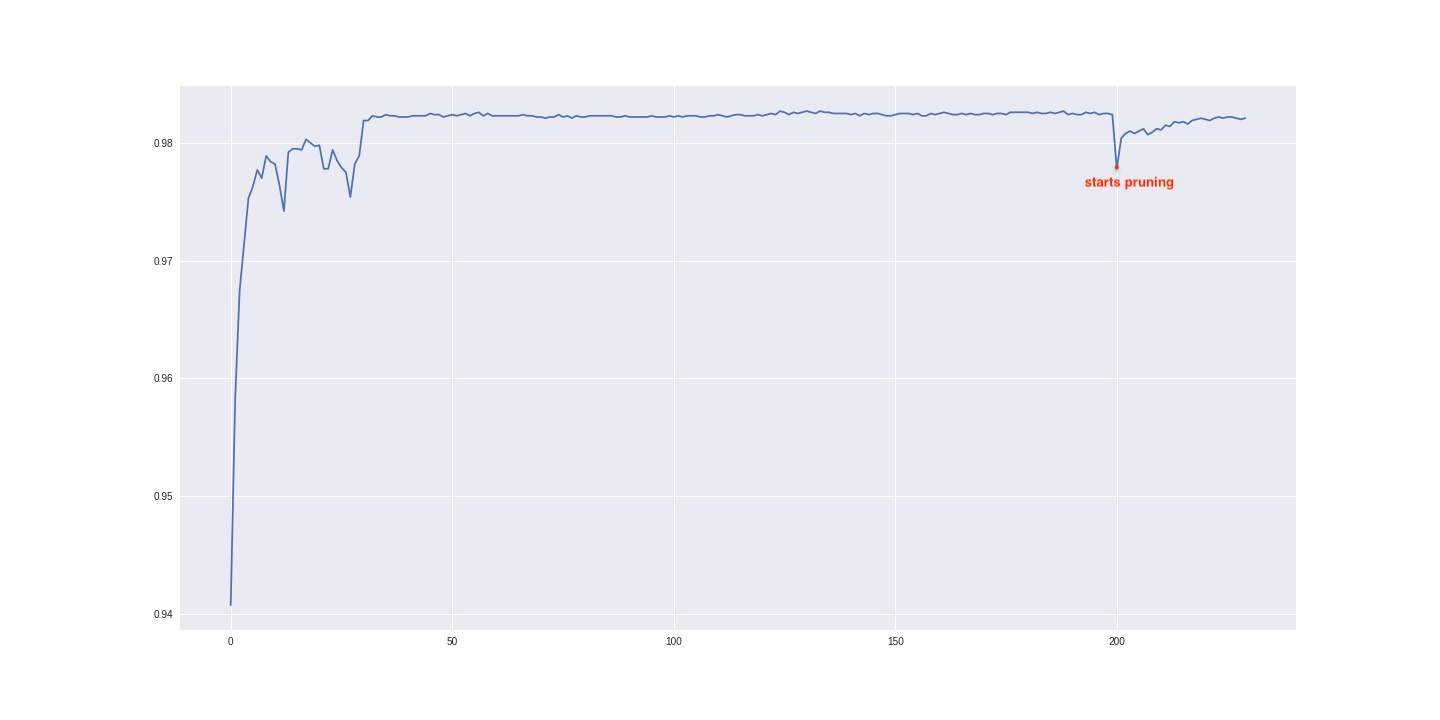
\includegraphics[width=90mm,scale=0.7]{accuracy-soft-threshold}
	\caption{Accuracy during the training for test 1 : when pruning starts at epoch 200 the accuracy slightly drops}
\end{figure}


\subsection{Test 2}
It is executed with LeNet300-100 with 200 epochs for normal training and 500 epochs for pruning, with higher hard thresholds : now the threshold is a constant value that is not multiplied by the standard deviation of the weights.\\In addition to this the loss function does not have the regularization terms.
\begin{table}[H]
\caption{Test 2 pruning results}
\label{my-label}
\begin{tabular}{|l|l|l|}
\hline
LAYER    & HARD THRESHOLD & ZERO WEIGHTS     \\ \hline
fc1      & 0.25         & 234521 on 235200 \\ \hline
fc1 bias & 0     & 0 on 300        \\ \hline
fc2      & 0.25          & 29030 on 30000   \\ \hline
fc2 bias & 0.0      & 0 on 100       \\ \hline
fc3      & 0       & 0 on 1000      \\ \hline
fc3 bias & 0         & 0 on 10          \\ \hline
\end{tabular}
\end{table}
The accuracy before pruning is : 98.22\% and after is : 96.11\%.\\This is the final accuracy after the different quantization techniques with 2,5,8 bits are applied after the pruning:
\begin{table}[H]
\caption{Test 2 quantization accuracy}
\label{my-label}
\begin{tabular}{|l|l|l|l|}
\hline
QUANTIZATION & 2-BITS  & 5-BITS  & 8-BITS  \\ \hline
Linear       & 31.39\% & 95.74\% & 96.11\% \\ \hline
Forgy        & 44.14\% & 93.31\% & 95.99\% \\ \hline
Dense        & 60.80\% & 95.63\% & 96.08\% \\ \hline
Kmeans++     & 31.10\% & 95.83\% & 96.13\% \\ \hline
\end{tabular}
\end{table}\begin{figure}[H]
	\hspace*{-1cm}
	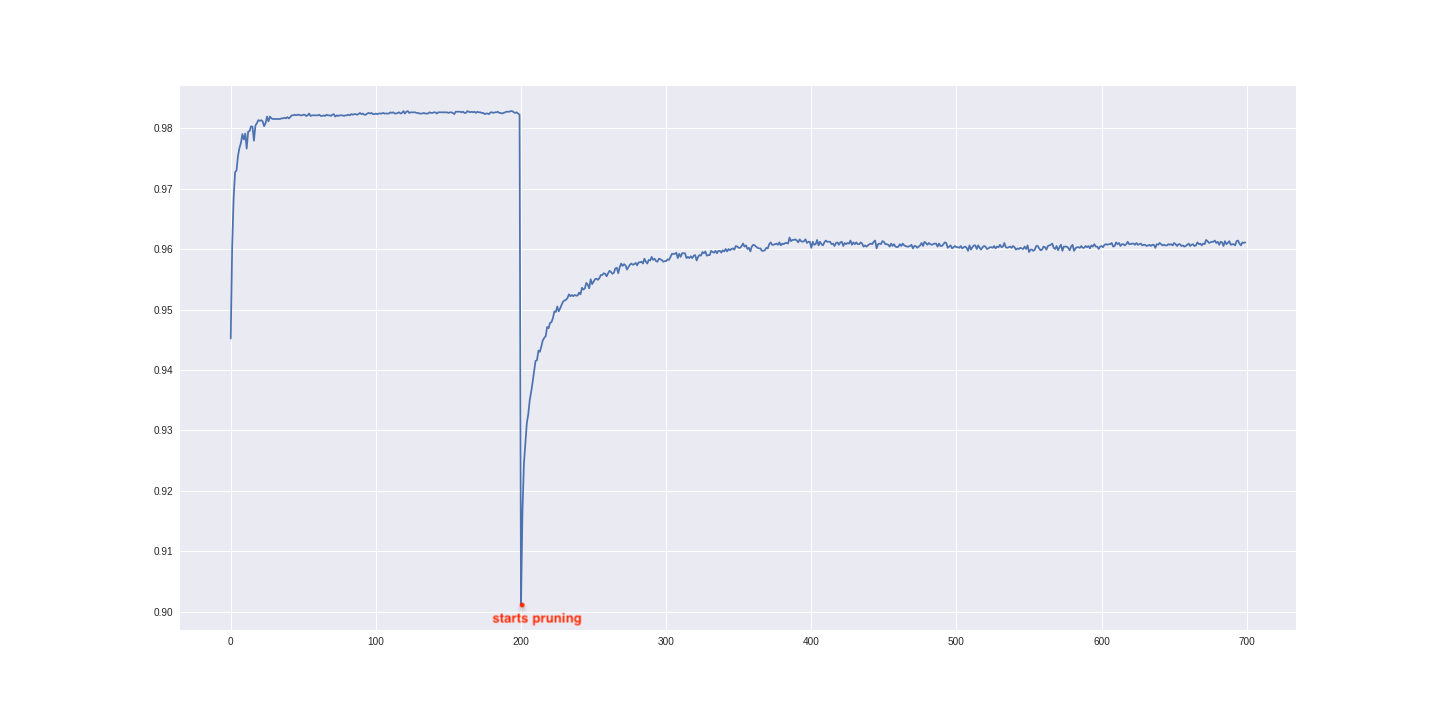
\includegraphics[width=90mm,scale=0.7]{accuracy-hard-threshold}
	\caption{Accuracy during the training for test 2}
\end{figure}
\subsection{Test 3}
It is executed with LeNet5 with 100 epochs for normal training and 30 epochs for pruning.\\It is important to stress the fact that as said before, to avoid the vanishing gradient problem, first the convolutional layers are pruned and then the dense layers (the same for the following test 4).
\begin{table}[H]
\caption{Test 3 pruning results}
\label{my-label}
\begin{tabular}{|l|l|l|}
\hline
LAYER    & THRESHOLD & ZERO WEIGHTS     \\ \hline
conv1      & 1         & 0 on 500 \\ \hline
conv1 bias & 0.1       & 0 on 20        \\ \hline
conv2      & 1         & 7826 on 25000   \\ \hline
conv2 bias & 0.1       & 0 on 50       \\ \hline
fc1      & 0.5       & 624960 on 627200      \\ \hline
fc1 bias & 0         & 256 on 256          \\ \hline
fc2 bias & 0         & 420 on 2560          \\ \hline
fc2 bias & 0         & 0 on 10          \\ \hline

\end{tabular}
\end{table}

The accuracy before pruning is : 99.24\% and after is : 99.29\%.\\This is the final accuracy after the different quantization techniques with 2,5,8 bits are applied after the pruning:
\begin{table}[H]
\caption{Test 3 quantization accuracy}
\label{my-label}
\begin{tabular}{|l|l|l|l|}
\hline
QUANTIZATION & 2-BITS  & 5-BITS  & 8-BITS  \\ \hline
Linear       & 99.17\% & 98.29\% & 99.29\% \\ \hline
Forgy        & 95.66\% & 99.30\% & 99.29\% \\ \hline
Density       & 99.16\% & 99.27\% & 99.28\% \\ \hline
Kmeans++     & 99.14\% & 99.28\% & 98.28\% \\ \hline
\end{tabular}
\end{table}\begin{figure}[H]
	\hspace*{-1cm}
	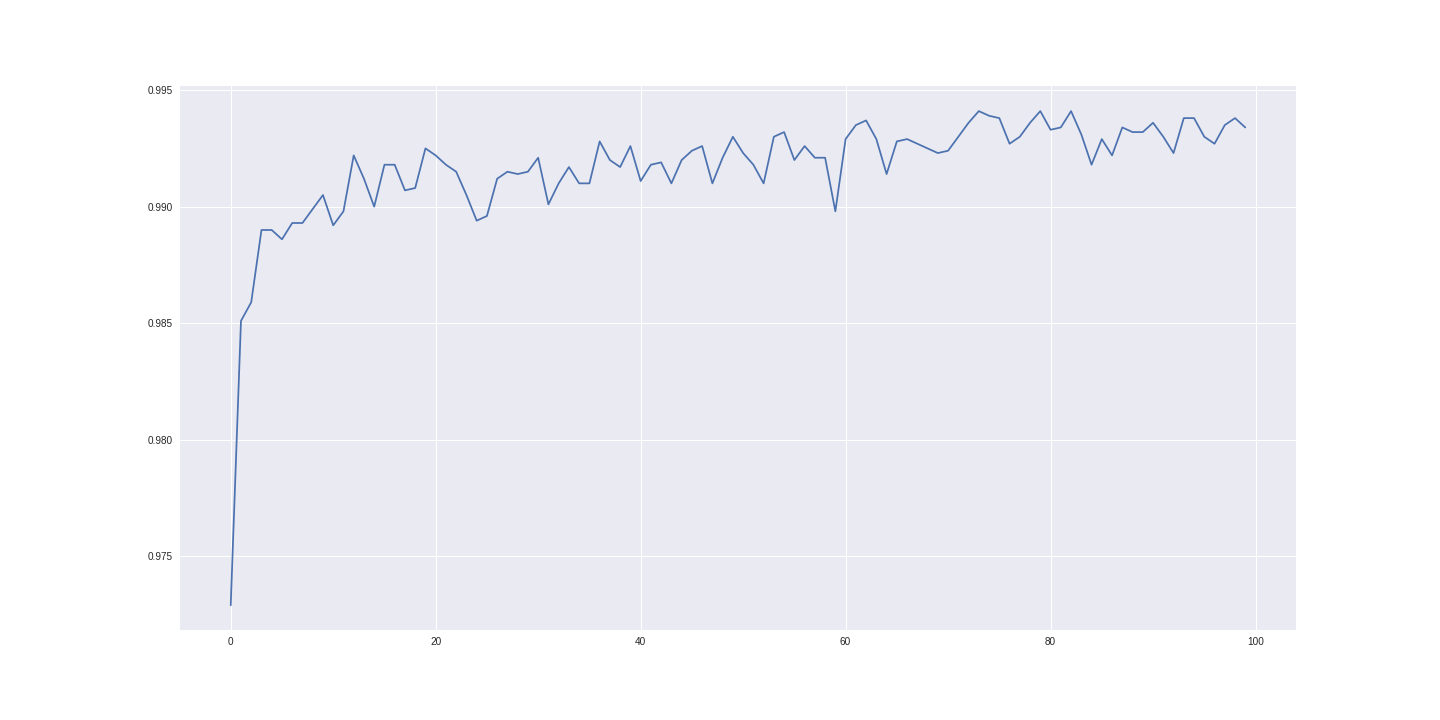
\includegraphics[width=90mm,scale=0.7]{accuracy-soft-threshold-conv}
	\caption{Accuracy during the training for test 3}
\end{figure}
\subsection{Test 4}
It is executed with LeNet35 with 70 epochs for normal training and 100 epochs for pruning, with higher hard thresholds.\\In addition to this the loss function does not have the regularization terms.
\begin{table}[H]
\caption{Test 4 pruning results}
\label{my-label}
\begin{tabular}{|l|l|l|}
\hline
LAYER    & HARD THRESHOLD & ZERO WEIGHTS     \\ \hline
conv1      & 0         & 0 on 500 \\ \hline
conv1 bias & 0       & 0 on 20        \\ \hline
conv2      & 0.25         & 24542 on 25000   \\ \hline
conv2 bias & 0      & 0 on 50       \\ \hline
fc1      & 0.5       & 620797 on 627200      \\ \hline
fc1 bias & 0         & 0 on 256          \\ \hline
fc2 bias & 0.1         & 982 on 2560          \\ \hline
fc2 bias & 0         & 0 on 10          \\ \hline

\end{tabular}
\end{table}
The accuracy before pruning is : 99.16\% and after is : 99.12\%.\\This is the final accuracy after the different quantization techniques with 2,5,8 bits are applied after the pruning:
\begin{table}[H]
\caption{Test 4 quantization accuracy}
\label{my-label}
\begin{tabular}{|l|l|l|l|}
\hline
QUANTIZATION & 2-BITS  & 5-BITS  & 8-BITS  \\ \hline
Linear       & 94.10\% & 99.09\% & 99.04\% \\ \hline
Forgy        & 96.29\% & 98.79\% & 99.01\% \\ \hline
Dense        & 97.57\% & 99.02\% & 99.03\% \\ \hline
Kmeans++     & 95.01\% & 99.02\% & 90.02\% \\ \hline
\end{tabular}
\end{table}\begin{figure}[H]
	\hspace*{-1cm}
	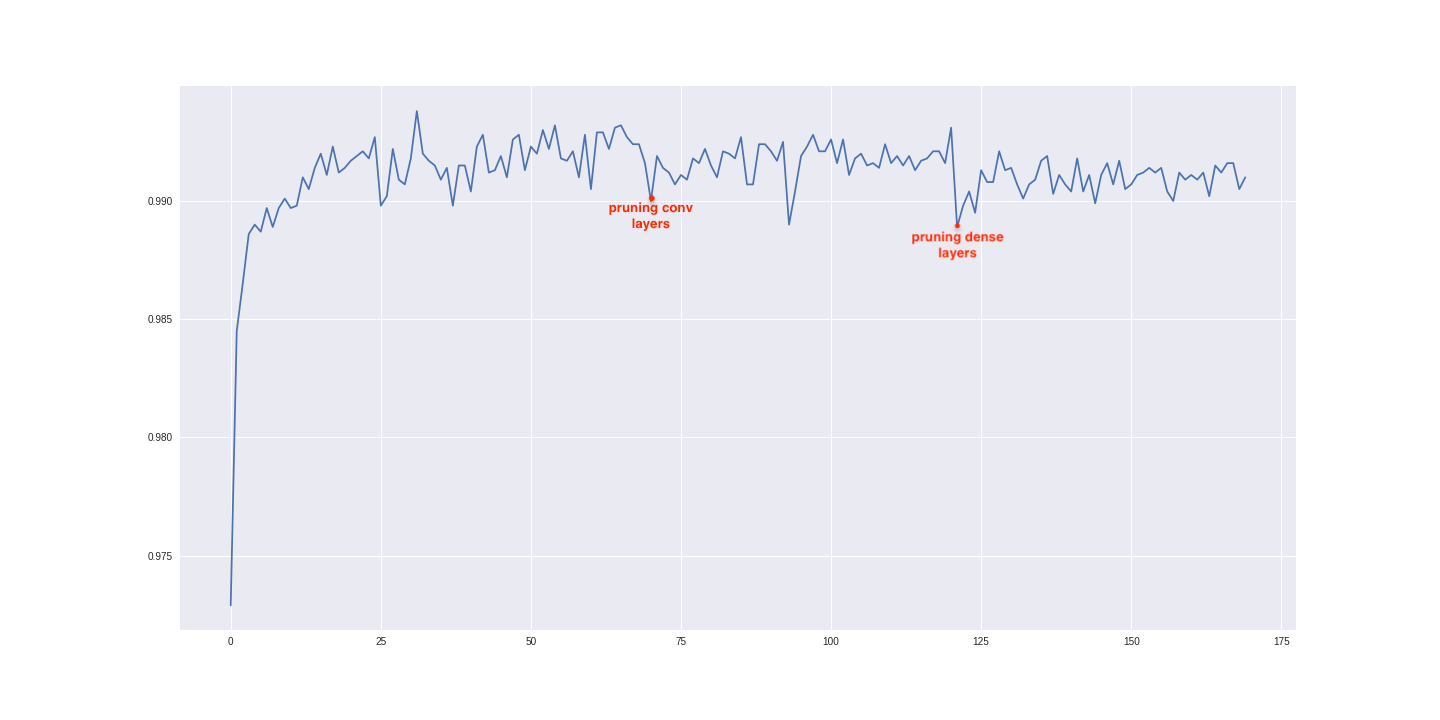
\includegraphics[width=90mm,scale=0.7]{accuracy-hard-threshold-conv}
	\caption{Accuracy during the training for test 4}
\end{figure}


\begin{thebibliography}{2}

\bibitem{p1}
  Song Han, Jeff Pool, John Tran, William J. Dally
  \textit{Learning both Weights and Connections for Efficient Neural Networks}
  
 \bibitem{p2}
  Song Han, Huizi Mao, John Tran, J. Dally
  \textit{DEEP COMPRESSION: COMPRESSING DEEP NEURAL NETWORKS WITH PRUNING, TRAINED QUANTIZATION AND HUFFMAN CODING}



\end{thebibliography}
\end{document}
